\section{\WatProvenance{}}\seclabel{WatProvenance}

\subsection{A Motivating Example}\seclabel{WatProvenanceExample}
\newcommand{\systemname}{ZardozBook} We claim that there is currently no
\emph{principled} way to reason about the causes of events in a heterogenous
distributed system. To best understand why, let's look at a simple example.
Consider the implementation of a Facebook-like social media application called
\systemname{}, illustrated in \figref{MeanComment}. \systemname{} users can
post statuses to their wall, and these status updates are only viewable by
their friends on the site. Users send requests to a load balancer which
forwards the requests to one of three weakly consistent Redis-backed
application servers: $s_1$, $s_2$, and $s_3$. These application servers store a
cache of \systemname{}'s data in Redis, and periodically they synchronize their
caches with a centralized Postgres database.

Consider a scenario in which Ava, a \systemname{} user, has a falling out with
Bob, a friend of hers on the site. Ava unfriends Bob and posts the status ``Bob
is a big jerk!'' to her wall, thinking that Bob will not see the status because
he is no longer her \systemname{} friend. Unfortunately, Bob later logs in to
\systemname{} and sees Ava's mean comment!

{\begin{figure}[ht]
  \centering
  \begin{tikzpicture}[xscale=1.5, yscale=0.75]

    % Icons.
    \tikzstyle{icon}=[inner sep=0pt]
    \node[icon] (woman) at (0, 3) {
\includegraphics[width=0.6cm]{figures/woman-crop.pdf}};
    \node[icon] (man) at (0, 1) {
\includegraphics[width=0.6cm]{figures/man-crop.pdf}};
    \node[icon] (router) at (1, 2) {
\includegraphics[width=0.6cm]{figures/router-crop.pdf}};
    \node[icon] (redis3) at (2, 1) {
\includegraphics[width=0.6cm]{figures/redis-crop.pdf}};
    \node[icon] (redis2) at (2, 2) {
\includegraphics[width=0.6cm]{figures/redis-crop.pdf}};
    \node[icon] (redis1) at (2, 3) {
\includegraphics[width=0.6cm]{figures/redis-crop.pdf}};
    \node[icon] (postgres) at (3, 2) {
\includegraphics[width=0.6cm]{figures/postgres-crop.pdf}};

    % Text
    \newcommand{\textsize}{\footnotesize}
    \node[anchor=south] at (woman.north) {\textsize Ava};
    \node[anchor=north] at (man.south) {\textsize Bob};
    \node[anchor=north, align=center] at (router.south) {\textsize{Load}\\\textsize{Balancer}};
    \node[anchor=south] at (redis1.north) {\textsize Redis};
    \node[anchor=south] at (postgres.north) {\textsize Postgres};

    % Labels.
    \tikzstyle{slabel}=[shape=circle, fill=white, fill opacity=0.7, text opacity=1, inner sep=0pt]
    \node[slabel] at (redis1) {$s_1$};
    \node[slabel] at (redis2) {$s_2$};
    \node[slabel] at (redis3) {$s_3$};

    % Edges.
    \tikzstyle{connection}=[stealth-stealth, line width=0.5pt]
    \draw[connection] (woman) to (router);
    \draw[connection] (man) to (router);
    \draw[connection] (router) to (redis1);
    \draw[connection] (router) to (redis2);
    \draw[connection] (router) to (redis3);
    \draw[connection] (postgres) to (redis1);
    \draw[connection] (postgres) to (redis2);
    \draw[connection] (postgres) to (redis3);
  \end{tikzpicture}
  \caption{Social media application}%
  \figlabel{MeanComment}
\end{figure}
}

Why did this happen? Here's an informal account.
\begin{itemize}
  \item
    Ava's request to unfriend Bob was forwarded to application server $s_1$ by
    the load balancer.
  \item
    Then, Ava's request to post the mean comment about Bob was forwarded to
    $s_2$.
  \item
    $s_2$ then pushed the comment to the Postgres repository.
  \item
    $s_3$ then issued a SQL query to the Postgres repository, pulling the
    latest data into its Redis cache. In doing so, it pulled in Ava's mean
    comment.
  \item
    Finally, when Bob logged in, his request was forwarded to $s_3$ which
    returned the mean comment.
\end{itemize}

We argue that there is no \emph{principled} way to go about discovering this
sequence of events. One possibility is to use causality, as described in
\secref{Background}. We could instrument our distributed system to record the
causal history of every event that takes place in the system. Then, we could
examine the causal history of Bob's request in an attempt to diagnose why Bob
was seeing Ava's mean comment. Unfortunately, this is not helpful. The causal
history of Bob's request includes \emph{every} event that causally precedes it,
whether or not the event is actually relevant. For example, the causal history
of Bob's request would include every single message that was received by server
$s_3$ prior to Bob sending his request, even those that do not involve Ava and
Bob. The problem is that causality is too coarse-grained. It fails to
incorporate any notion of a system's semantics as a means to filter out
irrelevant messages.  Instead, it returns a vast overapproximation of all the
events that \emph{might} cause an event instead of the events that
\emph{actually do} cause an event.

This might prompt us to try and apply ideas from data provenance. Unlike
causality, \whyprovenance{} does incorporate system semantics in order to
return the actual causes of a particular output of a query. Unfortunately,
\whyprovenance{} has two fatal flaws. First, \whyprovenance{} can only be
applied to relational algebra queries issued against a relation database. We
might be able to use \whyprovenance{} to debug $s_3$'s SQL query that was sent
to the Postgres database, but this is only one small piece of the puzzle.
Understanding why Bob saw Ava's mean comment requires us to reason about
messages that travel through our application servers, our redis servers, and
our load balancer. But, these are not relational databases, so we cannot apply
\whyprovenance{} to them. Second, \whyprovenance{} does not incorporate any
notion of time. \Whyprovenance{} operates under the assumptions of a
\emph{static} relational database, but our Postgres database, for example, is
not static. Thus, we cannot properly apply \whyprovenance{}, even to our
relational database.

Causality and data provenance are both insufficient to diagnose why Bob saw
Ava's mean comment. This leaves us with ad-hoc instrumentation as our only
means of debugging. We can instrument our system to log the messages that flow
through its components, and we can manually piece together the logs of every
server in our system. Besides being laborious, this ad-hoc instrumentation also
raises many questions. Which events should we log? And how do we identify the
``cause'' of an event? What do we even mean by ``the cause of an event''? Can
there be multiple ``causes'' or only one? Ideally, we would have a principled
and systematic way to answer these questions.

Enter \watprovenance{}.

% {\begin{figure}[ht]
  \centering
  \begin{tikzpicture}[scale=0.75]
    % Icons.
    \node[] (params) at (2, 0) {
\includegraphics[scale=0.5]{figures/sd-crop.pdf}};
    \node[] (laptop) at (4, 0) {
\includegraphics[scale=0.5]{figures/laptop-crop.pdf}};
    \node[] (worker) at (0, 0) {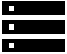
\includegraphics[scale=0.5]{figures/storage-crop.pdf}};

    % Text.
    \node[anchor=south, align=center] at (params.north) {Parameter\\Server};
    \node[anchor=north] at (worker.south) {Workers};
    \node[anchor=north] at (laptop.south) {Laptop};

    % Edges.
    \tikzstyle{connection}=[latex-latex, line width=1pt]
    \draw[connection] (worker) to (params);
    \draw[connection] (params) to (laptop);
  \end{tikzpicture}
  \caption{Distributed SGD}%
  \figlabel{ParameterServer}
\end{figure}
}
% We claim that there is currently no \emph{principled} way to reason about the
% causes of events in a heterogenous distributed system. To best understand why,
% let's look at a simple example. Consider a distributed implementation of sparse
% stochastic gradient descent (SGD) based on Hogwild!~\cite{recht2011hogwild}
% coordinated via a parameter server~\cite{li2014scaling}, as illustrated in
% \figref{ParameterServer}. We store our weight vector $x$ in a parameter server
% with each entry $x_i$ keyed by index $i$. We have a set of worker servers that
% periodically compute a gradient on a batch of the training data and push their
% updates to $x$ back to the parameter server. As the SGD executes, a data
% scientist's laptop periodically pulls the weights from the parameter server,
% computes the training error, and displays it to the data scientist so that they
% can monitor the progress of the SGD.
%
% {\begin{figure}[ht]
  \centering
  \begin{tikzpicture}[scale=0.75]
    % Icons.
    \node[] (params) at (2, 0) {
\includegraphics[scale=0.5]{figures/sd-crop.pdf}};
    \node[] (laptop) at (4, 0) {
\includegraphics[scale=0.5]{figures/laptop-crop.pdf}};
    \node[] (worker) at (0, 0) {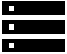
\includegraphics[scale=0.5]{figures/storage-crop.pdf}};

    % Text.
    \node[anchor=south, align=center] at (params.north) {Parameter\\Server};
    \node[anchor=north] at (worker.south) {Workers};
    \node[anchor=north] at (laptop.south) {Laptop};

    % Edges.
    \tikzstyle{connection}=[latex-latex, line width=1pt]
    \draw[connection] (worker) to (params);
    \draw[connection] (params) to (laptop);
  \end{tikzpicture}
  \caption{Distributed SGD}%
  \figlabel{ParameterServer}
\end{figure}
}


\subsection{\WatProvenance{}}

\subsection{Properties}

Begin by critiquing causality and why provenance. Now that we know what they are, this should be clear.

then state our objective. we would like to define provenance for arbitrary state machines.
definitions are asserted, not proved. we'll have to look at examples to get a sense
(1) sufficient and minimal
(2) any superset is sufficient
(3) set of witnesses, not just one thing

this is wat provenance
more examples

existince of witness
subsumption of why prov
